\chapter{Closing Remarks}

\section{Project Summary}

DX-SAHP shows potential in replacing natural gas heaters. The parts that have been selected for the project include a flat plate collector featuring an aluminum absorber plate, a copper serpentine manifold, and a single tempered glass glazing. The system’s subcomponents, i.e., the hermetically sealed variable speed compressor, the electronic expansion valve and the condenser are all interconnected via copper tubing. Sensors have also been selected for the control of the mechanism and to enable the acquisition of data during the testing phase. 

\medskip
The physical prototype was developed during this past semester and includes components such as the casing for the collector and a steel frame for the full assembly to sit on. The thermal collector was made solely by the team while the rest of the thermodynamic components were bought from vendors. An HVAC contactor helped braze the thermodynamic components to the solar thermal collector.

\medskip
The simulation results promise that the prototype will be able to meet the hot water needs of the average Canadian household. Once refrigerant charging is finished by a licensed professional, testing of the physical prototype can also be done to compare analytical and experimental results.

\section{Economic Analysis}

A typical water heater, both gas and electric powered, runs for 3-5 hours a day. In order to calculate the cost that will have to be paid to run the water heaters a simple equations may be used to \cite{energycalc}\cite{elecbill}:

\medskip
\begin{align}
    \dot E \times t \times r= TC
\end{align}

\medskip
where:
\\
$\dot E$ is the Energy per unit time
\\
$t$ is the hours in which the water heater is on
\\
$r$ is the cost per unit energy
\\
$TC$ is the total cost


\medskip
Knowing that as of 2021 electricity cost an average of 9.309\textcent/kWh and ENMAX 5-year average gas cost is \$4.09/GJ in Calgary, it can be calculated how much it costs run daily \cite{gasrate}\cite{ABenergy}.

\medskip
The heaters that are going to be used for comparison are Performance 40 Gal. Medium 6 Year 4500/4500-Watt Elements Electric Tank Water Heater as the electric water heater and Performance 40 Gal. Tall 6-Year 36,000 BTU Natural Gas Tank Water Heater for the gas heater \cite{electricheater}\cite{gasheater}. These are typically used in households today and will offer a good point of comparison.

\medskip
The estimated energy use of the natural gas heater per hour is 50000 Btu/hour and the wattage of the water heater 4500W.  Now the annually costs can be calculated.

\medskip
\textbf{Gas Heater:}
\begin{align}
    50000\frac{btu}{h}\times\ddfrac{1.0551\times10^{-6}GJ}{btu}\times5h\times\frac{\$4.09}{GJ} = \nicefrac{\$1.07}{day}=\nicefrac{\$393.78}{year}
\end{align}

\medskip
\textbf{Electric Heater:}
\begin{align}
    \ddfrac{4500W\times\nicefrac{\$0.13378}{kWh}\times 5h}{1000} = \nicefrac{\$3.01}{day}=\nicefrac{\$1098.67}{year}
\end{align}

\medskip
Meanwhile, the solar thermal water heater that was designed only needs 1kW at most (in winter conditions) to run. Using the same calculation for the electric water heater it can be estimated how much it will cost to run annually if it is assumed that the DX-SAHP runs for an average of 6 hours a day.

\medskip
\textbf{DX-SAHP:}
\begin{align}
    \ddfrac{1000W\times\nicefrac{\$0.13378}{kWh}\times 6h}{1000} = \nicefrac{\$0.80}{day}=\nicefrac{\$292.98}{year}
\end{align}

\medskip
As seen, the DX-SAHP design costs a similar amount per day as a gas water heater but is just as if not more environmentally friendly as an electric water heater. Using the initial cost, the payback period can be calculated when comparing it to a typical gas and electric water heater.


\medskip
\begin{table}[H]
\centering
\caption{Initial Costs for Water Heaters}
\rowcolors{2}{gray!20}{white}
\begin{tabular}{|P{45mm}|P{45mm}|P{45mm}|}
    \hline
    \rowcolor{orangeRed}
     Gas Water Heater & Electric Water Heater & DX-SAHP \\
    \hline
    \$569 & \$439 & \$5066.81 \\
    \hline
\end{tabular}
\end{table}

\medskip
The DX-SAHP has a higher initial cost in comparison to the heaters since it has all the components such as the collector, the frame, condenser and piping. What should be considered is that some of the parts were provided by sponsor, free of cost, so the price used does not truly reflect the cost of the system.

\medskip
Knowing all the initial costs we can graph the data:

\medskip
\begin{figure}[H]
    \centering
    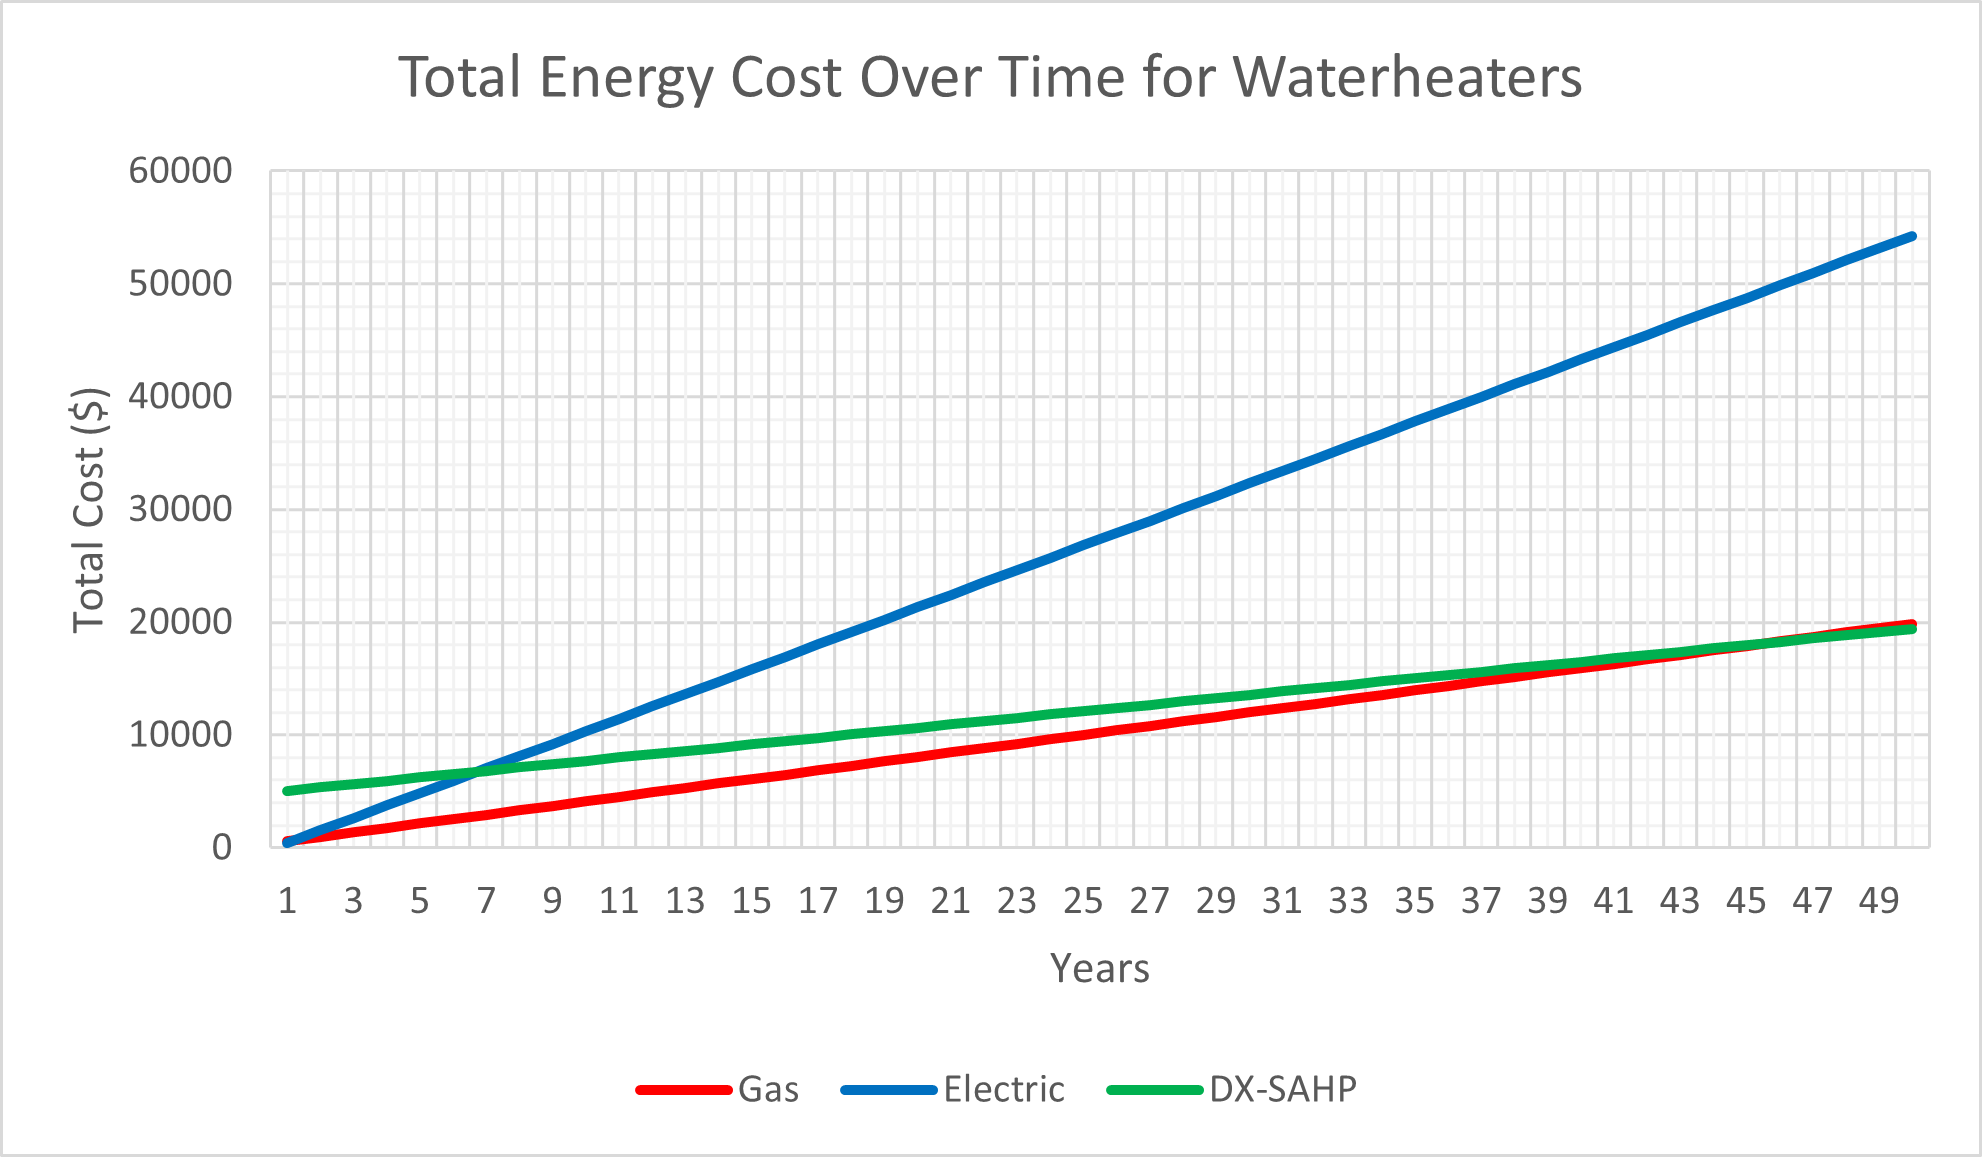
\includegraphics[width=12.5cm]{images/economic_analysis.png}
    \caption{Total Costs for Water Heaters}
\end{figure}

\medskip
The payback period is when the DX-SAHP line intersects with another projected energy cost. As seen in the graph above, the payback period when comparing it to gas fired water heaters is around 24 years while the payback period for gas is around 9 years.

\medskip
Another way to verify the payback period is to use this equation below \cite{PBperiod}:

\begin{align}
    PaybackPeriod = \frac{InvestmentCost}{AnnualCashFlow_{ave}}
\end{align}

\medskip
The average annual cash flow can be obtained by looking at how much is saved per year when comparing DX-SAHP to electric and gas-powered water tank heaters. Knowing that it costs \$393.78 and \$762.85 a year for gas and electric powered water tank heaters respectively, the average annual cash flow can be found by subtracting the annual cost of DX-SAHP (\$204.40) to find how much is saved. This results in an average annual cash flow of \$189.38 and \$558.45 when comparing it to gas and electric powered respectively. The calculations are as follows for the payback period:

\medskip
\textbf{Gas:}
\begin{align}
    \frac{\$ 5066.81}{\nicefrac{\$ 100.80}{year}} = 50.26years
\end{align}

\medskip
\textbf{Electric:}
\begin{align}
    \frac{\$ 5066.81}{\nicefrac{\$ 805.70}{year}} = 6.29years
\end{align}

\medskip
Since the solar collector brings in 1.81 kWh per day of heat, the amount of money that can be saved by using a solar collector instead of a heat pump can be determined.

\medskip
\textbf{Gas:}
\begin{align}
    1.81kWh\times\nicefrac{0.0036GJ}{kWh}\times\frac{\$4.09}{GJ} = \nicefrac{\$0.03}{day}=\nicefrac{\$9.73}{year}
\end{align}

\medskip
\textbf{Electric:}
\begin{align}
    1.81kWh\times\frac{\$0.13378}{kWh} = \nicefrac{\$0.24}{day}=\nicefrac{\$88.38}{year}
\end{align}

\medskip
Gas may seem to be a better choice economically, but this does not consider the environmental and safety concerns associated with it. DX-SAHP is more sustainable when comparing it to gas fired water heaters and since water heaters get replaced every 8-12 years, it is more economical than electric water heaters in most scenarios \cite{lifeheater}.

\section{Suggestions for Design Improvements}

The provided compressor is a fixed speed type which is not efficient as a variable frequency compressor, but the latter could not be sourced for the system configurations as they currently stand.  If a variable frequency drive is to be added, at least a 3-phase motor would be required, and thus the compressor would have to be switched out.

\medskip
Using a copper absorber plate rather than an aluminum one would also greatly benefit the design. If proceeding with copper tubing as well, the brazing process could achieve a higher thermal performance of the system with minimized air gaps and the process itself would be much easier, as copper-to-copper brazing is relatively simple.

\medskip
The current state of the prototype does not have the glass glazing that was mentioned before. This was mainly due to costs and the possibility of injury when handling heavy glass. For a future iteration, the glass can be modified to be safer to handle and possibly cheaper in costs.

\medskip
The municipal water supply in Calgary is quite hard. For future iterations, a demineralizer or water softener may be required to reduce the amount of scale build up in the coaxial condenser coil, hot water tank, and hot water pump. This will ensure that the system will be continuously operating at optimal conditions which will extend its lifetime.

\medskip
The prototype as of now has to be manually shut on and off. This is adequate as a baseline because the prototype is mainly going to be used for testing purposes. In the future, however, a control element to turn the system on and off automatically can be integrated. The control element would turn off the full system once the water in the tank is homogeneously at 55 \textdegree C.

\section{Project Management Lessons Learned}

\medskip
Throughout the process of this project some lessons can be learned about project management and how to improve further.

\medskip
Firstly, a schedule needs to be clearly outlined. This allows the team to remain on track for completion. By using a combination of soft and hard deadlines for certain tasks, it can ensure that everything is completed within a timely manner.

\medskip
Secondly, ensuring that tasks are distributed fairly and evenly. This allows for everyone to contribute equally to the project and prevents a single person from being overburdened. It also prevents that likelihood of burnout throughout the team.

\medskip
Lastly, open and honest communication is necessary for a healthy environment and for the collaboration of the team. By having the ability to speak freely about any issues or problems that may arise, it allows the team to tackle the problem in an efficient manner and to maintain morale.